\chapter{Introduction}
Technological studies in the fields of \gls{adas} and \gls{ad} have been growing in the past decades in the auto-mobile industry and in the academic environment. 

It is important in \gls{ad} and \gls{adas} to implement machine learning methods so that the vehicles recognize what objects are in their surroundings. Therefore, a necessity to have data that instructs the vehicles appears. Data labelling is the solution to create datasets that will serve as input to learning algorithms.

This thesis is focused on the research of a method to register data into labels using a camera and \gls{lidar} sensors in ATLASCAR 2, so that the vehicle can later create a model of the objects it will detect and track.

The objects detected by ATLASCAR 2 are to be used in deep-learning algorithms. The acquired data must be large enough so that the models for each object can be well defined.

This dissertation will also improve some previous work, namely the calibration of the camera installed in ATLASCAR 2. In addition to the calibration, a tool for image labeling and tracking of objects will be developed. This tool will be used to gather image templates while tracking objects in the camera video. 

\section{ATLAS Project}

ATLAS is a project developed by the Group of Automation and Robotics at the Department of Mechanical Engineering of the University of Aveiro, Portugal. The mission of the ATLAS project is to develop and enable the proliferation of advanced sensing and active systems designed for implementation in automobiles and affine platforms. Advanced active systems being improved, or newly developed, use data from vision, laser and other sensors. The ATLAS project has vast experience with autonomous navigation in controlled environments and is now evolving to deal with real road scenarios. To ensure that the developments are meeting the ATLAS project mission statement, a full sized prototype, the ATLASCAR 1, has been equipped with several state of the art sensors (\cite{LARlabs}). Currently, ATLASCAR 2 is the new full sized prototype being used for research. The ATLASCAR 2 is also equipped with \gls{lidar} sensors and a camera.

\subsection{History}

The ATLAS Project was created in 2003 and began with robots developed to participate at \gls{ad} competitions taking place at Portuguese National Robotics Festival. From this project, three small-sized platform robots were built (figure \ref{fig:atlasproto}). These robots were very successful having won prizes in some of the robotics competitions. 


\begin{figure}[htp]
	
	\centering
	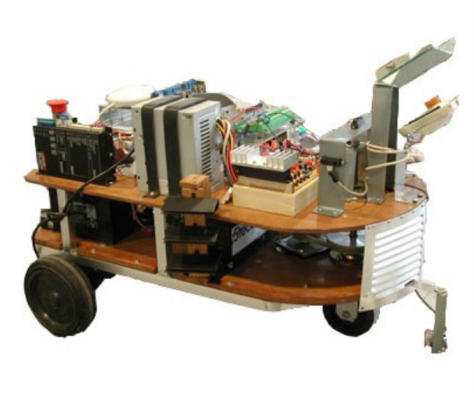
\includegraphics[width=.3\textwidth]{capintro/imgs/atlas1}\hfill
	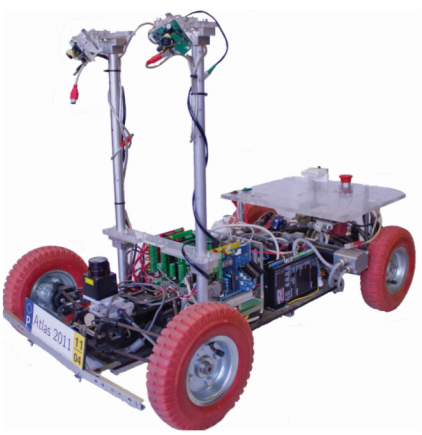
\includegraphics[width=.3\textwidth]{capintro/imgs/atlas2000}\hfill
	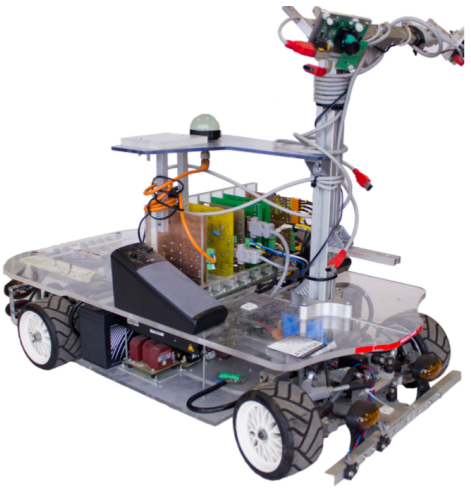
\includegraphics[width=.3\textwidth]{capintro/imgs/atlasmv}
	
	\caption{ATLAS project small-sized prototypes}
	\label{fig:atlasproto}
	
\end{figure}

As the project grew, it has evolved into full-sized prototypes: the ATLASCARs. ATLASCAR 1 (figure \ref{fig:atlascar1}) is the first full-sized platform and it is based on a Ford Escort Station Wagon. The ATLASCAR 1 is well equipped with several \gls{lidar} sensors and a camera. Data about its environment is gathered by the scanners which is then processed building perception into the car. With perception is possible for the vehicle to actuate allowing the car to move autonomously. 

\begin{figure}[htp]
	
	\centering
	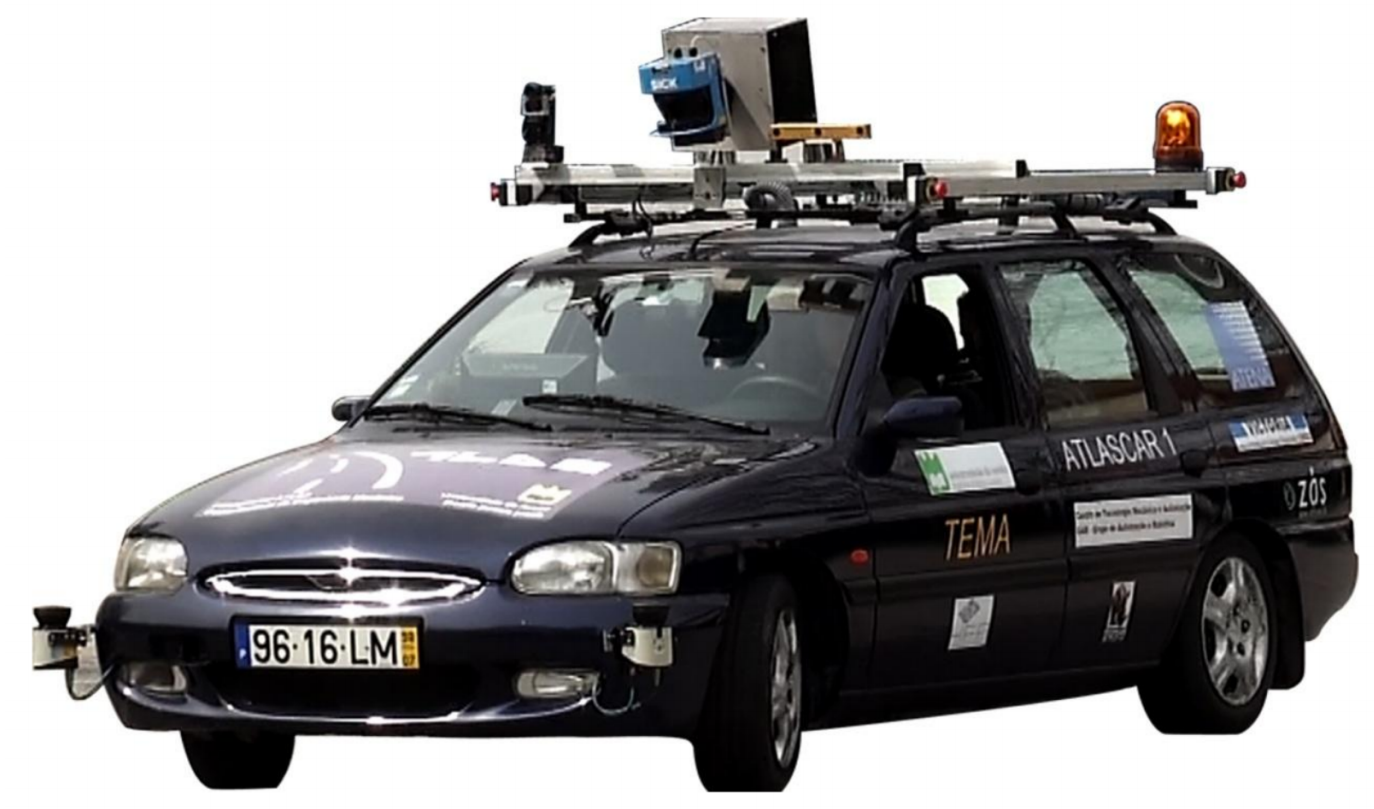
\includegraphics[width=0.9\textwidth]{capintro/imgs/atlascar1}
	
	\caption{ATLASCAR 1 based on the Ford Escort platform}
	\label{fig:atlascar1}
	
\end{figure}

The ATLASCAR 1 brought successful results. In the end, the vehicle was able to move and execute maneuvers autonomously in small and controlled places. The ATLASCAR 1 was then replaced by a more recent vehicle. The ATLASCAR 2 (figure \ref{fig:atlascar1}) is the new full-sized platform of the ATLAS project and it is based on a Mitsubishi i-MiEV. This is the vehicle used for research in this dissertation. The ATLASCAR 2 is well equipped with various \gls{lidar} sensors and a camera. It is also a full electric vehicle which will be easier to modify, test and control. 

\begin{figure}[htp]
	
	\centering
	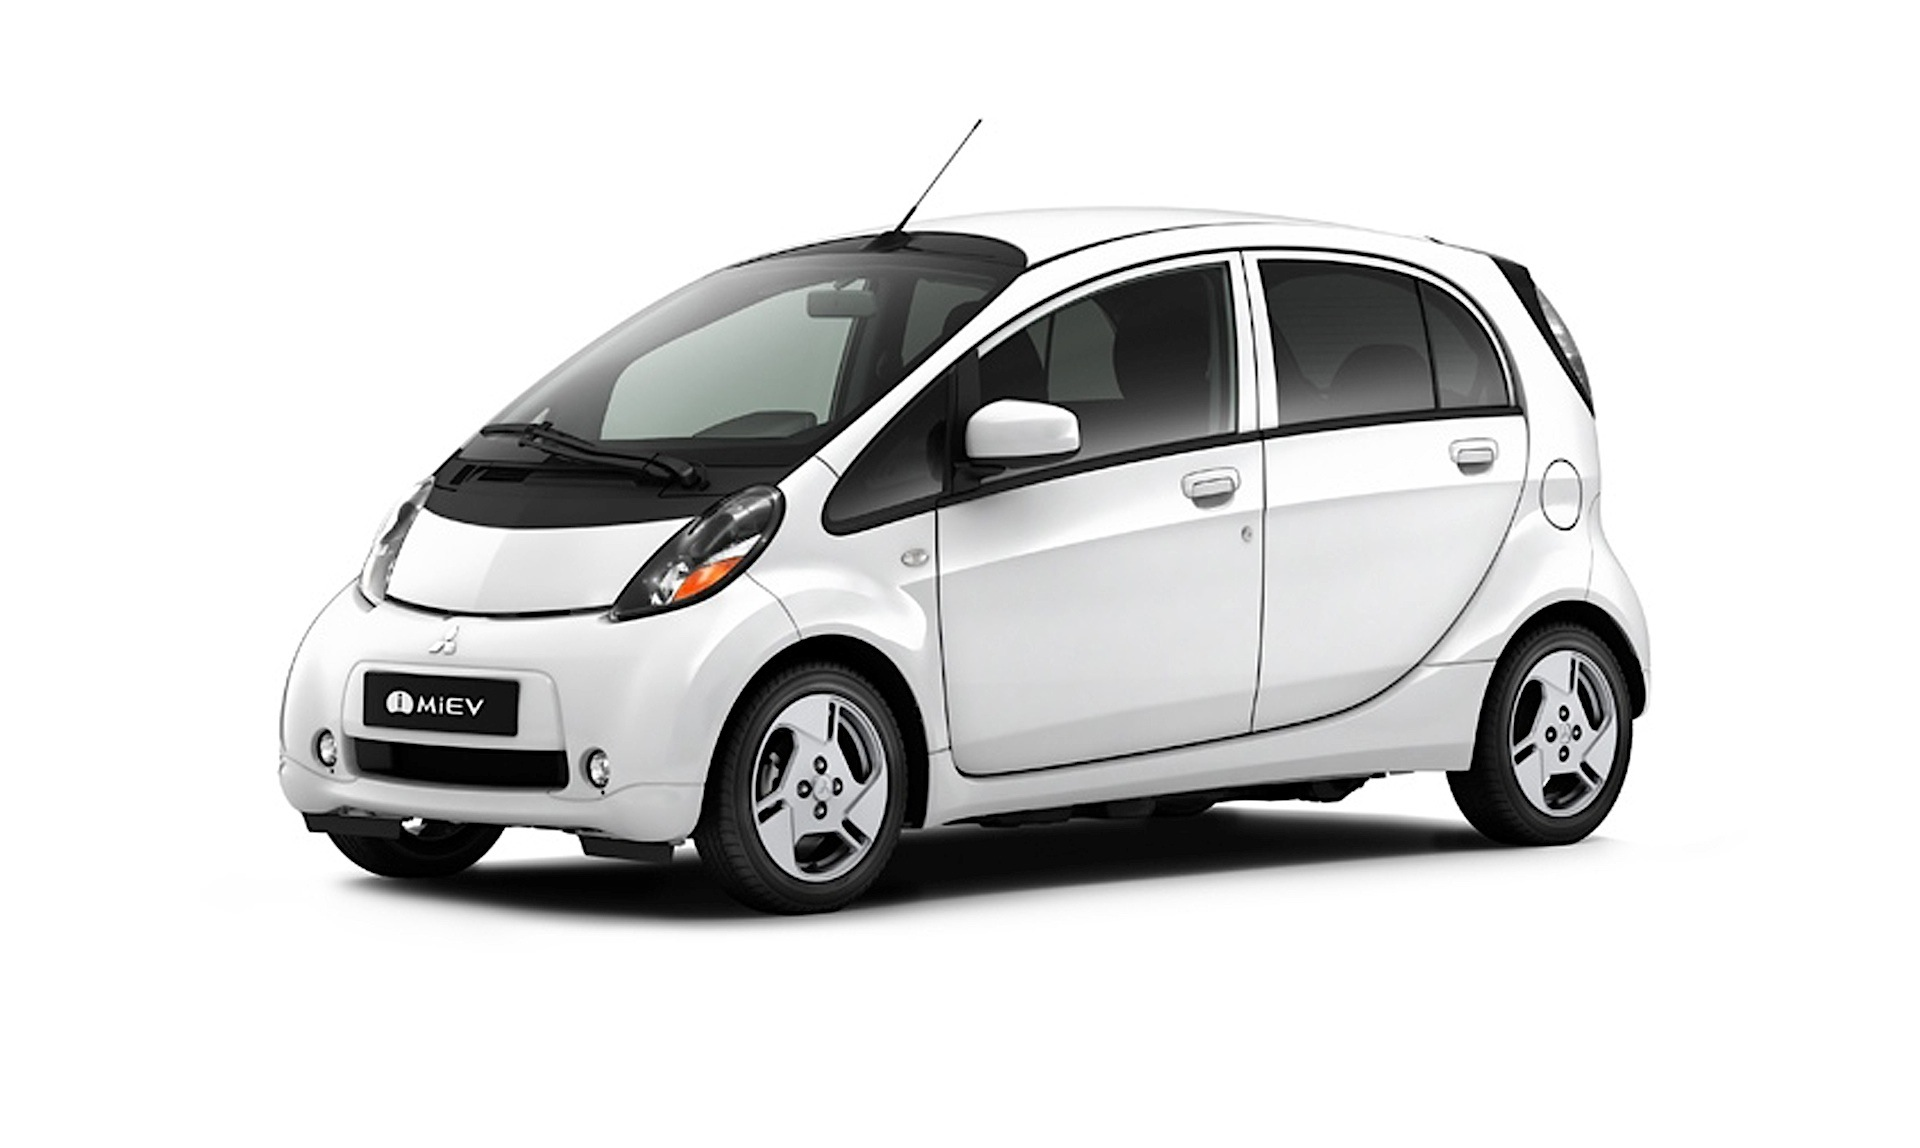
\includegraphics[width=0.9\textwidth]{capintro/imgs/imiev}
	
	\caption{Mitsubishi i-MiEV platform where ATLASCAR 2 is based}
	\label{fig:atlascar2}
	
\end{figure}


\section{Motivation}
The ATLASCAR 2 is the new platform of the ATLAS Project. The car has a mounted infrastructure for \gls{lidar} scanners and a vision-based sensors. With a fully equipped vehicle, the data from the surroundings is ready to be received and processed. 

To use multiple sensors at the same time in a system, it is fundamental that these devices are properly calibrated. The LIDAR sensors and the camera can be submitted into an extrinsic calibration in order to find their position relatively to a reference sensor. A fully calibrated system is important to deal with the data acquired from each sensor. Planar LIDAR sensors need to know their position between each other so that a full pointcloud of all sensors can be created for visualization purposes or for any end.

\gls{ad} and \gls{adas} often make use of machine learning. Deep learning algorithms utilize neural and convolutional networks for images and range-based sensor data. In the fields of machine learning, images are often used as input templates to create object models. In an image sequence it is possible to track an object and obtain samples of the \gls{roi} where the target is. This way it is possible for an algorithm to automatically recognize an object.

While registering the position of the objects in an image sequence, it is important to tell what those objects are. Labelling is the act to classify objects in a certain group. As the annotation is done, when selecting an object, the user should enter a label that identifies the target making it easy for the learning algorithm to recognize to object afterwards.

The objective and importance of tagging samples of images with a label is to assign metadata in the form of a keyword in order that later an application can retrieve this information and easily construct a database. However, most labelling for images is currently done with non optimized rudimentary procedures like capturing samples of the \gls{roi} manually and frame by frame, making this process slow and obsolete.

In the end of this dissertation, the ATLASCAR2 will have a labelling system that fuses images retrieved from the camera with the laser data, creating a semi automatic object tracking system that offers the possibility to retrieve various image template sequences and store metadata about them. This metadata contains, for instance, the label, object related identification markers and position of the object in the image and in the real world relatively to the ATLASCAR2.

\section{Objectives}
The objectives for this dissertation are, firstly, to improve the calibration of the camera, in particular regarding the detection of the ball by the camera in the existing multi-sensor calibration package developed using the \gls{ros}. Secondly, the development of other \gls{ros} package used for semi-automatic detection and labelling of objects in the field of view.

The calibration package was already developed by \cite{VieiradaSilva2016}. The methods used to detect the ball in the camera image were basically filtering values from the \gls{hsv} color space. There are methods that can make this detection more robust that will be explained in this thesis. 

To complete the goal of object tracking and image labelling there were a set of techniques and libraries used. In vision-based sensors, the object tracking algorithm is based on template matching methods and in range-based sensors the tracking is accomplished by the \gls{mtt} library developed by \cite{SoaresDeAlmeida2016a}.

\section{Document Structure}

This document is composed by seven chapters including the introduction. In the second chapter, the related work previously done on ATLASCAR 2 will be described as well as a literature review will detail the most significant milestones on the history of autonomous driving and a research on image labelling datasets will be presented and analyzed. 

In the third chapter, the experimental structure of this dissertation will be described depicting the hardware (ATLASCAR2 and sensors) and the software (\gls{ros}, \gls{lartk} and \gls{pcl}). 

In the forth chapter, the implementation of the calibration node will be explained presenting its features, the base algorithm and how the calibration package was modified in order to improve the ball detection. 

In the fifth chapter, the detection, tracking and labelling node development will be taken into account, firstly by describing how the image tracking is done, then clarifying how to track objects using the \gls{lidar} sensors and finally using both the image and sensor data to obtain maximum precision. In this chapter the outputted datasets will also be presented and some extra features used to aid in the labelling will also be described. 

In the sixth chapter, it will be presented the results of the ball detection and integration with the calibration package will be shown and the outcome of the labelling node will also be analyzed using some datasets produced by the same. 

The final chapter the conclusions of this thesis are presented and some future work related to the scope of this dissertation is proposed.

